\chapter{Methodology and results }
\label{ch2}


\section{Data source}
personal financial data is taken from kaggle.com. Below are the Columns with description:

\begin{figure}[h]
    \centering
    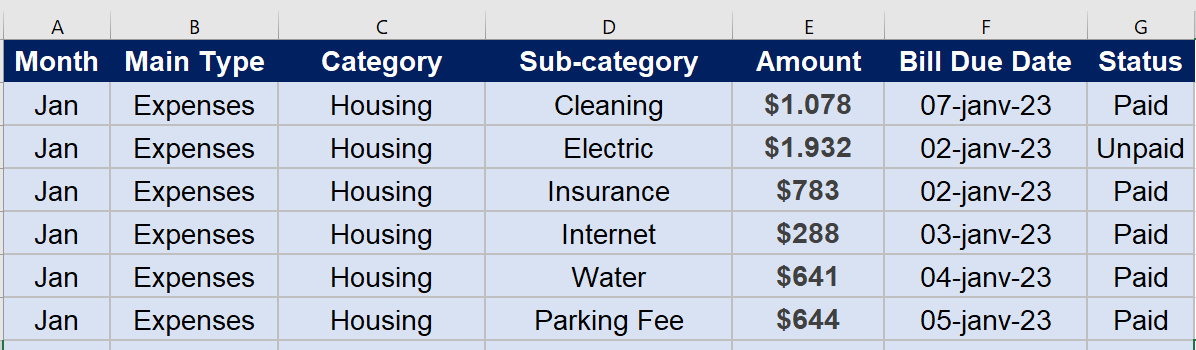
\includegraphics[width=6.0in, height=3.0in]{Figure/Capture d’écran (504).png}
    \caption{Excel raw data}
    \label{fig:enter-label}
\end{figure}

\textbf{Month:} This column refers to the month in which the financial transaction or activity occurred. It provides a chronological timeline for tracking expenses and income over time.

\textbf{Main type:} This column categorizes the type of financial transaction or activity. It could include both categories incomes and expenses.

\textbf{Category:} This column further categorizes the financial transaction or activity into broader categories such as  under  housing, transportation, food, etc.

\textbf{Sub-category: }This column provides more specific details about the nature of the financial transaction or activity within the broader category. For example, under the housing category, sub-categories could include rent, property taxes, insurance, etc.

\textbf{Amount:} This column records the monetary value associated with the financial transaction or activity. It represents the amount of money spent, earned, saved, invested, or owed.

\textbf{Bills due date: }This column indicates the due date for bills or payments associated with the financial transaction or activity.

Status: This column reflects the current status  of the financial transaction or activity. 

\section {How to upload raw data into Power BI}
To create the personal financial dashboard, I followed these steps to upload my data:

\begin{enumerate}
    \item First, I downloaded and installed Power BI Desktop on my computer.
    \item Once it was installed, I opened the application and followed these steps:
    \begin{enumerate}
        \item I clicked on the "Get Data" button to start importing my data.
        \item I chose "Excel Workbook" as the source of my data.
        \item Then, I browsed my computer to find my raw data file and selected the required sheets.
        \item After selecting the sheets, I clicked on "Transform" to proceed.
        \item This opened the Power Query Editor window where I could review and modify my data.
        \item I made sure to check all data types from each table to ensure accuracy.
        \item Finally, I clicked on "Close \& Apply" to import and apply the changes to my data.
    \end{enumerate}
\end{enumerate}

Now, my base data is ready to be used in Power BI.


\section{Data Analysis Expressions (DAX) }
Data Analysis Expressions (DAX) is a query programming language that is used throughout
Microsoft Power BI for creating calculated columns, measures, and custom tables. It is a
collection of functions, operators, and constants that can be used in a formula, or expression, to
calculate and return one or more values.

\section{ Key feature and DAX Queries}
I have created multiple measures with DAX query:

\begin{enumerate}
    \item \textbf{Visualization of monthly expenses by category:}
\\\ Total Expenses = \text{CALCULATE}([\text{Total Amount}], \text{FILTER}('Main Data', 'Main Data'[Main Type]="Expenses"))
\begin{figure}[h]
    \centering
    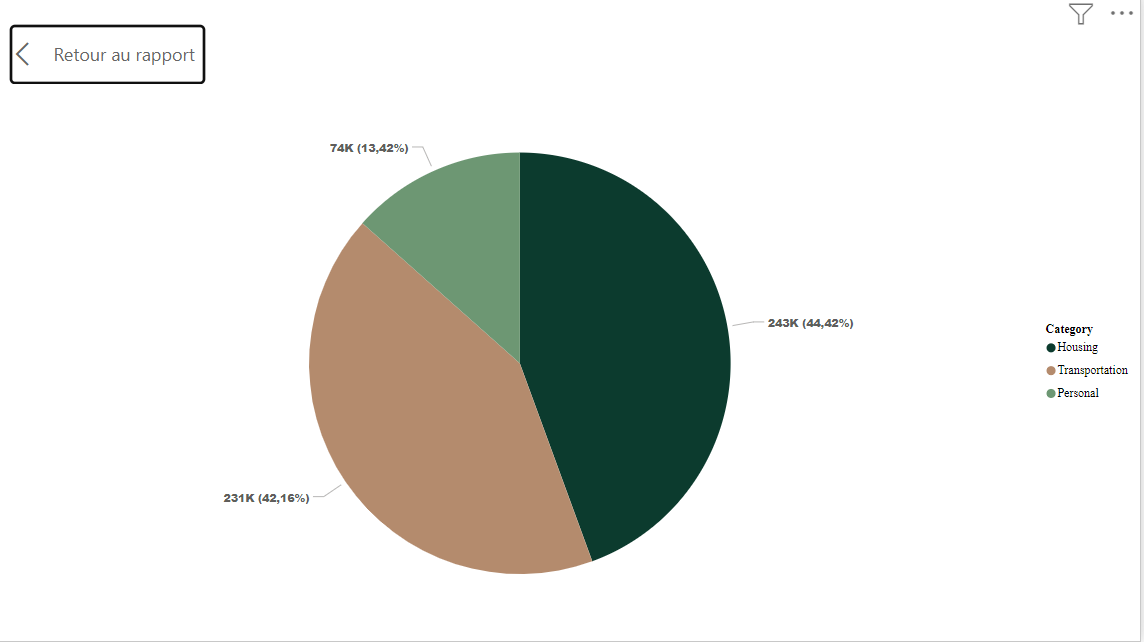
\includegraphics[width=5.0in, height=3.0in]{Figure/expenses-per category.png}
    \caption{Expenses per month by category}
    \label{fig:enter-label}
   
\end{figure}
\\\

 \textbf{ \item {Tracking of monthly income :}}
\text{Total Income} = \text{CALCULATE}([\text{Total Amount}], \text{FILTER}('Main Data', 'Main Data'[Main Type]="Income"))
\\\ 
\text{Side Income} = \text{CALCULATE}([\text{Total Amount}], \text{FILTER}('Main Data', 'Main Data'[Category]="Side Income"))
\\\ 
\text{Main Income} = \text{CALCULATE}([\text{Total Amount}], \text{FILTER}('Main Data', 'Main Data'[Category]="Main Income"))
\begin{figure}[h]
    \centering
    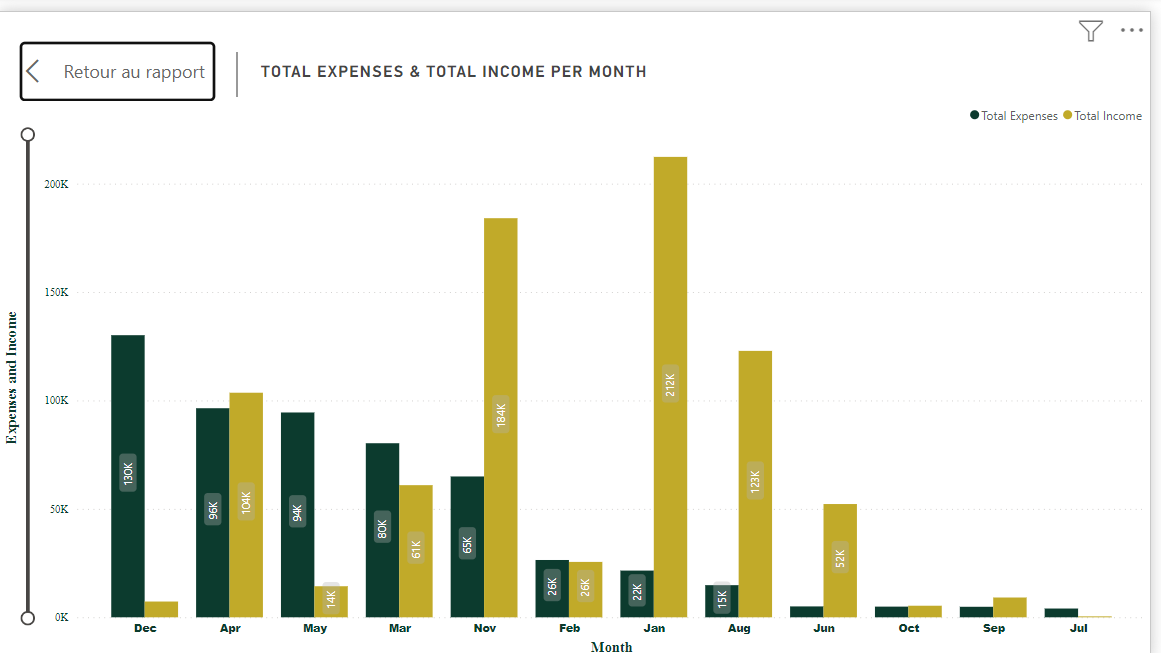
\includegraphics[width=5.0in, height=3.0in]{Figure/expenses-income-per-month.png}
    \caption{Expenses and  income per month}
    \label{fig:enter-label}
   
\end{figure} 


 \item \textbf{Analysis of the net evolution of wealth over time:}

\text{Net Wealth} = 
\text{CALCULATE}(
    \text{SUM}('Main data'[Amount]),
    'Main data'[Main type] = "income"
) - 
\text{CALCULATE}(
    \text{SUM}('Main data'[Amount]),
    'Main data'[Main type] = "expenses"
)
\begin{figure}[h]
    \centering
    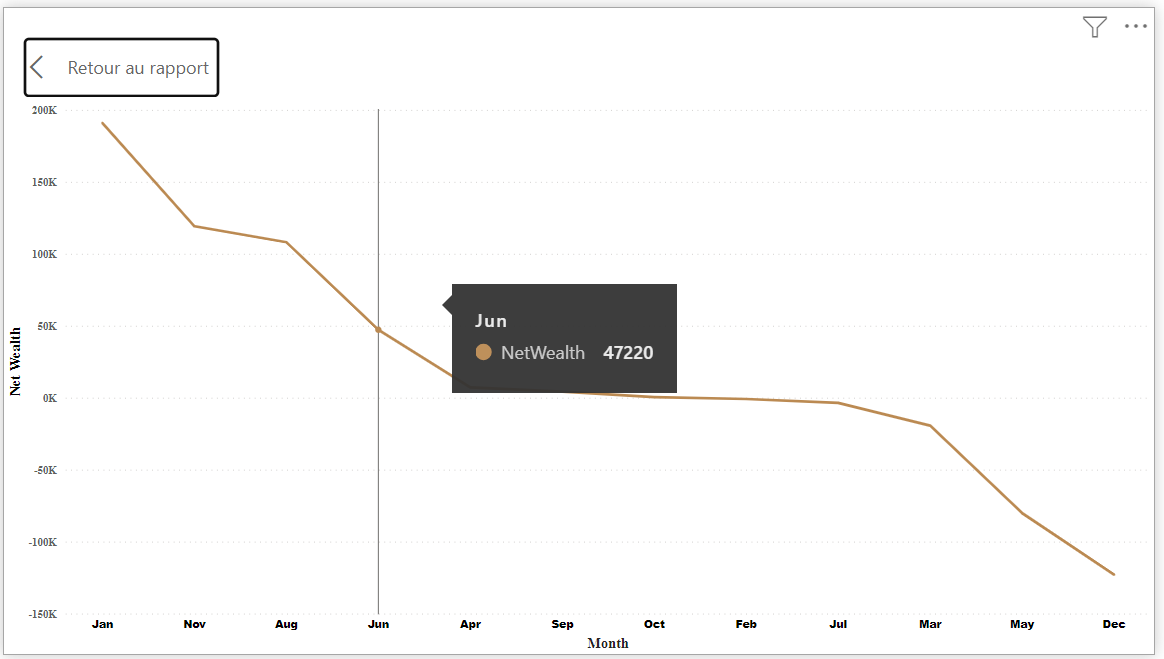
\includegraphics[width=5.0in, height=3.0in]{Figure/Netwealth per month.png}
    \caption{Nat wealth analysis}
    \label{fig:enter-label}
   
\end{figure}












\end{enumerate}



